\documentclass[12pt]{article}

\usepackage[utf8]{inputenc}
\usepackage{geometry}
\geometry{a4paper,scale=0.75}
\linespread{1.5}
\usepackage{graphicx} 
\usepackage{float} 
\usepackage{subfig} 
\usepackage{enumerate}
\usepackage{enumitem}
\usepackage{amsmath}
\usepackage{array}
\usepackage{booktabs}
\usepackage{multirow}
\usepackage{amsfonts}
\usepackage[english]{babel}
\usepackage{amsthm}
\usepackage{dcolumn}
\usepackage{multicol}
\usepackage{stfloats}
\usepackage{lscape}
\usepackage[figuresright]{rotating}
\RequirePackage{pdflscape}
\usepackage[toc,page]{appendix}
\usepackage{geometry}
\usepackage{longtable}
\usepackage{comment}
\usepackage{xcolor}

% -------- enumerated sub-labels (a), (b), … --
\usepackage{enumitem}
\setlist[enumerate,1]{label=(\alph*),ref=\alph*}
% ---------------------------------------------

\usepackage{hyperref}
\hypersetup{hidelinks,
	colorlinks=true,
	allcolors=black,
	pdfstartview=Fit,
	breaklinks=true}
\usepackage{csquotes}
\usepackage{natbib}
\bibliographystyle{apalike}
\newtheorem{definition}{Definition}
\newtheorem{theorem}{Theorem}
\newtheorem{proposition}[theorem]{Proposition}
\newtheorem{lemma}[theorem]{Lemma}
\newtheorem{corollary}[theorem]{Corollary}
\newtheorem*{remark}{Remark}
\newtheorem{example}{Example}
\newtheorem{exercise}{Exercise}
\newtheorem{assumption}{Assumption}[section] % number within sections


\begin{document}

\begin{center}
    ECON 3123: Macroeconomic Theory I\\
    {\large \textbf{Tutorial Note 7: Labour Market and Phillips Curve}}\\
    Teaching Assistant: Harlly Zhou
\end{center}

\subsection*{A Simple Model of the Labour Market}
\paragraph{Price Determination} Consider a production function
\[Y = AN.\]
The \textbf{marginal product of labour} (MPL) is $\frac{\partial Y}{\partial N} = A$. Suppose that the cost of hiring an extra worker is $W$. Then the marginal cost of production is $\frac{W}{A}$. Let $m$ be the markup (due to monopolistic power). Then the price level will be
\[ P = (1+m)\frac{W}{A}.\]

\paragraph{Wage Determination} Assume that the nominal wage is
\[W = A P^e F(u,z),\]
where $A$ is the MPL, $P^e$ is the expected price level, and $F$ is a function decreasing in unemployment rate $u$, and increasing in $z$, a variable capturing all other factors.

\paragraph{Natural Rate of Unemployment} From the price determination equation, we have
\[\frac{W}{P} = \frac{A}{1+m}.\]
From the wage determination equation, \textbf{since $P^e=P$ in the medium run}, we have
\[\frac{W}{P} = AF(u,z).\]
In a $\left(u, \frac{W}{P}\right)$ diagram, the pricing curve is a horizontal line, and the wage curve is a downward-sloping curve, as is shown in Figure \ref{fig:wu_01}. The equilibrium unemployment rate that is reached by the two curves is called the \textbf{natural rate of unemployment}.

\begin{figure}[htp]
    \centering
    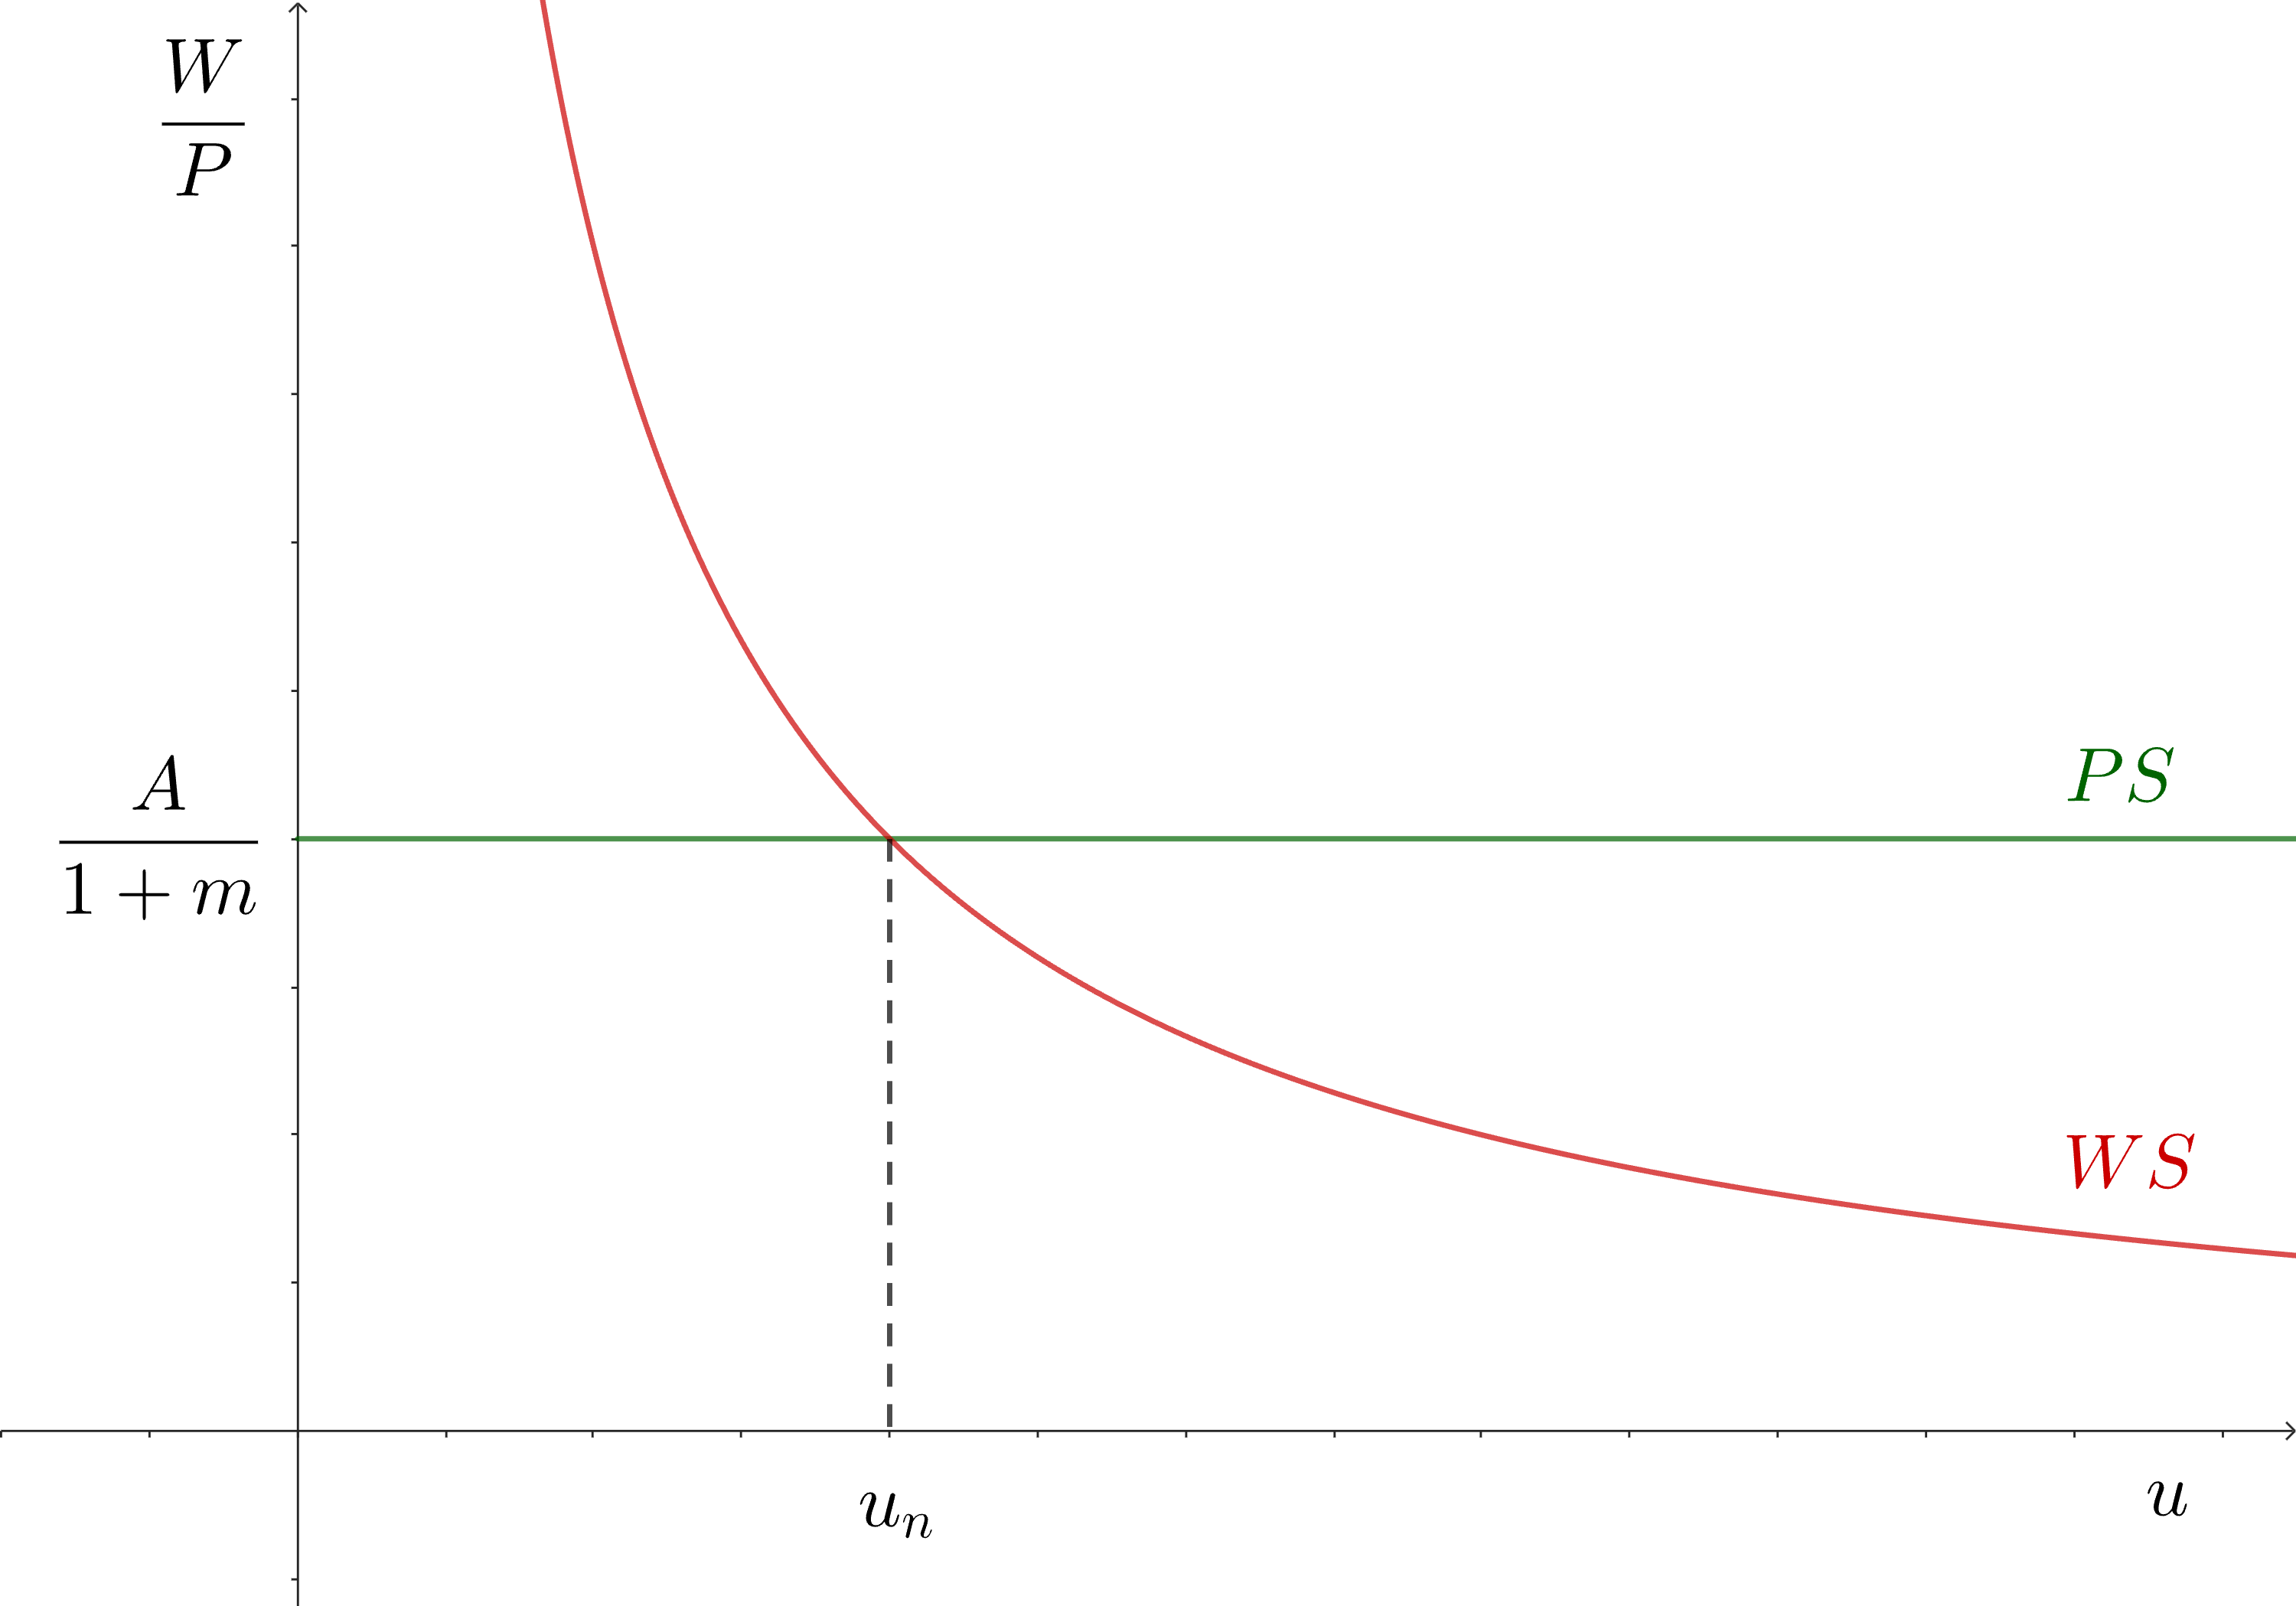
\includegraphics[width=0.6\textwidth]{wu_01.png}
    \caption{Natural Rate of Unemployment}
    \label{fig:wu_01}
\end{figure}

\begin{example}
    Consider a linear production function
    \[Y = AN.\]
    Let the wage setting equation be
    \[\frac{W}{P^e} = A F(u,z),\]
    where $z$ is the union power and
    \[F(u,z) = 1 - \alpha u_t + \phi z_t.\]
    Suppose that the union can bargain for a real minimum wage at
    \[\frac{W}{P}\geq\underline{w}_t = \omega z_t\]
    \begin{enumerate}[label=(\arabic*)]
        \item When the minimum wage is not hit, find out the equilibrium real wage and write the natural rate of unemployment (not by log approximation) as a function of $z_t$ and parameters.
        \vspace{60pt}
        \item Suppose that the constraint binds. Find the natural rate of unemployment as a function of $z_t$ and parameters.
        \vspace{60pt}
        \item Find the threshold for $z_t$ where the minimum wage constraint binds. Denote it as $\bar{z}$.
        \vspace{60pt}
        \item When the constraint binds, how does the natural rate of unemployment change with union power? Explain the economic intuition.
        \vspace{60pt}
    \end{enumerate}
\end{example}



\begin{exercise}
    Chapter 7, Question 5 in Blanchard, Olivier (2021), \textit{Macroeconomics}, 8th ed., Pearson.
\end{exercise}

\subsection*{Deriving the Phillips Curve}
Recall that the labour market equilibrium is the intersection of
\begin{align*}
    \text{Wage setting: }\,\,&\frac{W}{P^e} = AF(u,z)\\
    \text{Price setting: }\,\,&P = (1+m)\frac{W}{A}.
\end{align*}
Combining the two curves, we obtain
\[P = P^e(1+m) F(u,z).\]
Assume that
\[F(u,z) = 1-\alpha u +z.\]
Then
\[P_t = P^e_t(1+m) (1-\alpha u_t +z).\]
Dividing both sides by $P_{t-1}$, we obtain
\[\log\frac{P_t}{P_{t-1}} = \log\frac{P^e_t}{P_{t-1}} + \log (1+m) + \log (1-\alpha u_t +z).\]
By approximation, we have the \textbf{Phillips curve}:
\[\pi_t = \pi^e_t + (m+z) - \alpha u_t.\]

\paragraph{Original Phillips Curve}
Assume that inflation does not persist: $\pi^e = \bar{\pi}$,meaning that past inflation rates are not informative to predict new inflation. Then the Phillips curve becomes
\[\pi_t = (\bar{\pi}+m+z) - \alpha u_t.\]
Denote $\beta := \bar{\pi}+m+z$. Then we have
\[\pi_t = \beta - \alpha u_t.\]
However, there are periods when this original Phillips curve is not supported by the data.

\paragraph{Accelerationist Phillips Curve}
Assume that inflation persists: $\pi^e = \pi_{t-1}$, meaning that people use the inflation from the past period as the indicator of expected inflation. Then the Phillips curve becomes
\[\pi_t = \pi_{t-1} + (m+z) - \alpha u_t.\]
Denote $\gamma := m+z$. Then we have
\[\Delta \pi_t = \gamma - \alpha u_t.\]
The period now fits.

\paragraph{Inflation Expectations}
As in the previous two versions of PC, we have different methods to form expectations for inflation. Combining the two methods, we can assume that
\[\pi_t = (1-\theta)\bar{\pi} + \theta\pi_{t-1}.\]

\paragraph{Implications from Phillips Curve}
Disinflation can be costless. Suppose the central bank would like to decrease the inflation rate. Then it can announce a lower targeted inflation in period $t-1$ so that $\pi_t^e$ is lowered. However, it does not change any policy when it reaches period $t$. By doing so, the government can decrease the inflation costlessly. However, the problem is that the central bank announcement will have less credibility, which makes it harder to implement committed monetary policy (\textit{i.e., } a monetary policy path).


\begin{exercise}
    Chapter 8, Question 5 in Blanchard, Olivier (2021), \textit{Macroeconomics}, 8th ed., Pearson.
\end{exercise}

\subsection*{Natural Rate of Unemployment Revisited}
Recall the the natural rate of unemployment is the rate at which $P=P^e$, \textit{i.e.}, the labour market is at medium-run equilibrium. Since $P=P^e$, we also have $\pi=\pi^e$ in medium-run equilibrium. Then the PC becomes
\[0 = (m+z)-\alpha u_n,\]
which yields
\[u_n = \frac{m+z}{\alpha}.\]
Then the PC (not at equilibrium) can be rewritten as
\[\pi_t - \pi_t^e = -\alpha (u_t - u_n).\]

\paragraph{Wage Indexation}
\textbf{Wage indexation} is a provision that automatically increases wages in line with inflation. Suppose that there is a $\lambda$ proportion of indexed contracts. Then we have two types of wage settings:
\begin{align*}
    \text{Indexed Wage: }\, & W_1 = A P_t F(u_t,z)\\
    \text{Normal Wage: }\, & W_2 = A P^e_t F(u_t,z).
\end{align*}
Then the price setting becomes
\[P_t = (1+m)\frac{\lambda W_1 + (1-\lambda) W_2}{A} = [\lambda P_t + (1-\lambda)P_t^e] F(u,z)(1+m),\]
which yields the following PC curve:
\[\pi_t = [\lambda\pi_t + (1-\lambda)\pi_t^e]-\alpha(u_t-u_n).\]
Rearranging the terms, we get
\[\pi_t-\pi_t^e = -\frac{\alpha}{1-\lambda}(u_t-u_n).\]

\begin{exercise}
    Chapter 8, Question 6 in Blanchard, Olivier (2021), \textit{Macroeconomics}, 8th ed., Pearson.
\end{exercise}


\begin{example}[New Keynesian Phillips Curve]
    Consider a production function
    \[Y_t = A N_t\]
    where $Y_t$ is the output, $A$ is labour productivity, and $N_t$ is the labour. Let $P_t$ be the price level and $W_t$ be the nominal wage. Denote $p_t = \log P_t$ and $w_t = \log W_t$.
    \begin{enumerate}[label=(\arabic*)]
        \item Find the price setting equation in log terms.
        \vspace{60pt}
    \end{enumerate}
    Normalize the price setting equation so that $p_t = w_t$. Suppose that we have two types of workers. Type 1 workers sign contracts in odd years and type 2 workers sign contracts in even years. The contract is valid for two years, within which the nominal wage is fixed. Each type of workers consists of half of the total labour. At year $t$, denote the wage of workers who get contract renewed by $x_t$. Hence, those who get contract renewed in the year before $t$, that is, $t-1$, have wage $x_{t-1}$. All terms are in log.
    \begin{enumerate}[label=(\arabic*),resume]
        \item Find the expected nominal log wage of year $t+1$ at year $t$.
        \vspace{36pt}
        \item Find the avergae log price level in year $t$.
        \vspace{36pt}
        \item Assume that the discount factor is 1. Find the average real log wage over the period of a constract renewed from year $t$, denoted by $\omega_t$.
        \vspace{60pt}
    \end{enumerate}
    Denote the log output by $y_t$. Assume that $\omega_t = k y_t$ ($0<k<1$).
    \begin{enumerate}[label=(\arabic*),resume]
        \item Show that
        \[p_t = \frac{1}{4}(2p_t + \mathbb{E}_t p_{t+1} + p_{t-1} + \eta_t) + \frac{k}{2}(y_t + y_{t-1}),\]
        where $\eta_t = \mathbb{E}_{t-1} p_t - p_t$.
        \vspace{80pt}
        \item Derive the New Keynesian Phillips Curve (NKPC):
        \[\pi_t = \mathbb{E}_t \pi_{t+1} + \eta_t + 2k(y_t + y_{t-1}).\]
        \vspace{60pt}
        \item Can the central bank decrease inflation costlessly? How?
        \vspace{24pt}
    \end{enumerate}
\end{example}

\begin{example}
    Consider the following production function
    \[Y = A \log N.\]
    The wage determination equation, in the medium run equilibrium, is
    \[\frac{W}{P} = AF(u,z)\equiv A(1-\alpha u_t + z).\]
    \begin{enumerate}[label=(\arabic*)]
        \item Let $m$ be the markup. Write the price setting equation, \textit{i.e.,} write $P$ as a function of $N$.
        \vspace{24pt}
        \item Let the population $L$ be normalized to 1 and assume that it is constant. Find a quadratic equation characterizing the natural rate of unemployment. Which solution to the equation you should keep? Why?
        \vspace{24pt}
        \item Suppose that the labour productivity $A$ increases. Using a diagram, explain what happens to the new equilibrium real wage and the new natural rate of unemployment.
        \vspace{48pt}
        \item Derive the Phillips curve.
        \vspace{24pt}
        \item Write the accelerationist version of the Phillips curve. Compare it with
        \[\Delta \pi_t = \gamma - \alpha u_t.\]
        What is the difference? Where does it come from? Explain with economic intuition.
        \vspace{24pt}
        \item Find the natural rate of unemployment using the Phillips curve. Check your answer with part (2). Do they match? Rewrite the Phillips curve using the natural rate of unemployment.
        \vspace{48pt}
        \item Suppose that now half of the contracts are indexed. Write the Phillips curve equation.
        \vspace{48pt}
        \item What is the effect of wage indexation on the relation between inflation and unemployment?
        \vspace{24pt}
    \end{enumerate}
\end{example}

\end{document}